\begin{frame}
  \frametitle{Struktura překladače}
    \begin{itemize}
        \setlength\itemsep{1em}
        \item Lexikální analýza: \emph{scanner.c}
        \item Syntaktická analýza: \emph{parser.c}
        \item Syntaktická analýza: \emph{expression.c}
        \item Tabulka symbolů: \emph{symtable.c}
        \item Sémantická analýza: \emph{parser.c} a \emph{expression.c}
        \item Generování kódu: \emph{generate\_code.c} a \emph{builtIn.c}
    \end{itemize}
\end{frame}



\begin{frame}
  \frametitle{Lexikální analyzátor}
    \centering
    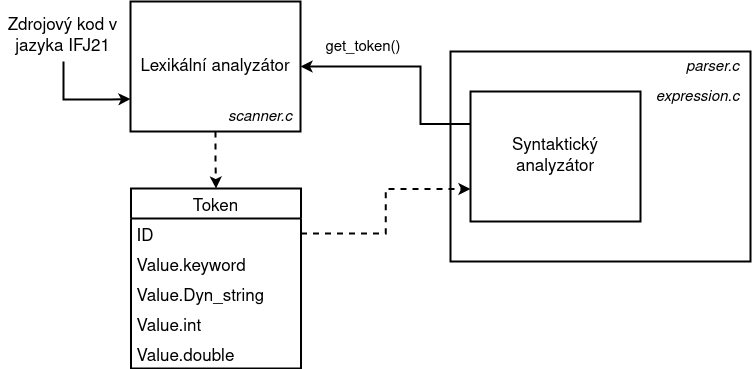
\includegraphics[scale=0.34,keepaspectratio]{img/DiagramLex.png}
  
  \vspace{1em}
  
    \begin{itemize}
        \item KA implementovaný přepínači
        \item Tokeny na vyžádání syntaktické analýzy
        \item Načtená data v atributech tokenu
        \item Řetězce uložené v \emph{dynamickém stringu}
    \end{itemize}
\end{frame}



\begin{frame}
  \frametitle{Syntaktická analýza shora dolů}
        \begin{itemize}
        \setlength\itemsep{1em}
            \item \emph{Rekurzivní} sestup
            \item Funkce vrací hodnotu odpovídající chybě
            \item \emph{Uložení pozice čtení} před rozhodovacím tokenem
            \item Předání řízení analýze zdola nahoru u výrazů
        \end{itemize}
    
    \vspace{1.5em}
    
        \begin{flushleft}
        \fontdimen2\font=0.4em
        \texttt{
        \emph{pos\_t} pos = \emph{fgetpos(}srcFile\emph{)}\newline\newline
        \textit{načtení tokenu a rozhodnutí}\newline\newline
        \emph{fsetpos(}pos\emph{)}}
        \end{flushleft}
\end{frame}



\begin{frame}\frametitle{Syntaktická analýza zdola nahoru}
  \begin{columns}
    \column{0.5\textwidth}
    \begin{itemize}
    \setlength\itemsep{1em}
        \item \emph{Precedenční přístup}
        \item Zásobník terminálů a neterminálů
        \item Precedenční tabulka implementovaná \emph{2D polem}
        \item Výraz se vyhodnotí při přijetí neočekávaného tokenu
    \end{itemize}
    
    
    \column{0.5\textwidth}
    \centering
    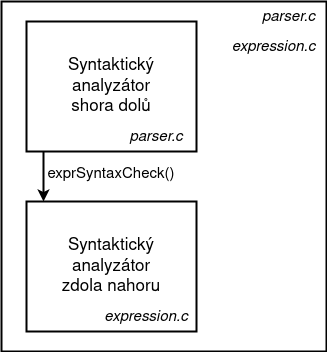
\includegraphics[scale=0.34,keepaspectratio]{img/DiagramSynt1.png}
    \end{columns}
\end{frame}



\begin{frame}
  \frametitle{Tabulka symbolů}
  \centering
  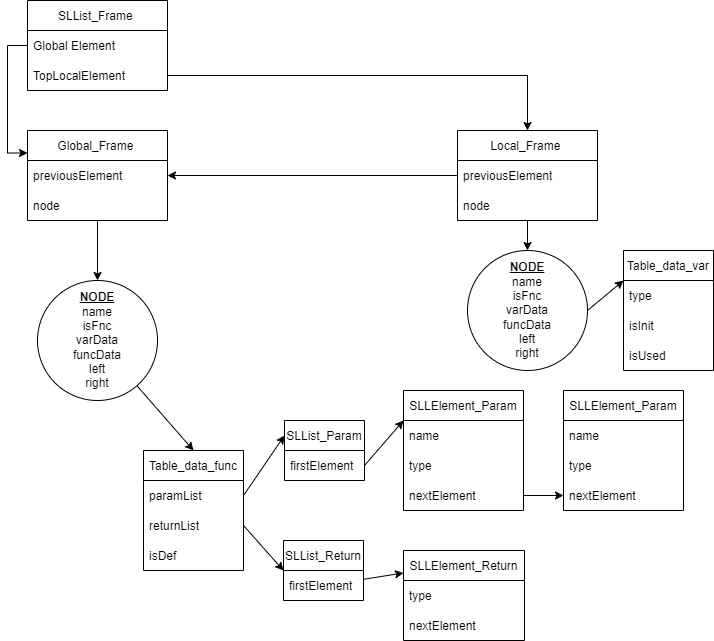
\includegraphics[scale=0.37]{img/Symtable.png}
\end{frame}



\begin{frame}\frametitle{Sémantická analýza}
    \begin{columns}
        \column{0.44\textwidth}
        \begin{itemize}
        \setlength\itemsep{1em}
            \item Doplněny k syntaktické analýze
            \item Zásobník na datové typy operandů
        \end{itemize}
        
        \column{0.56\textwidth}
        \centering
        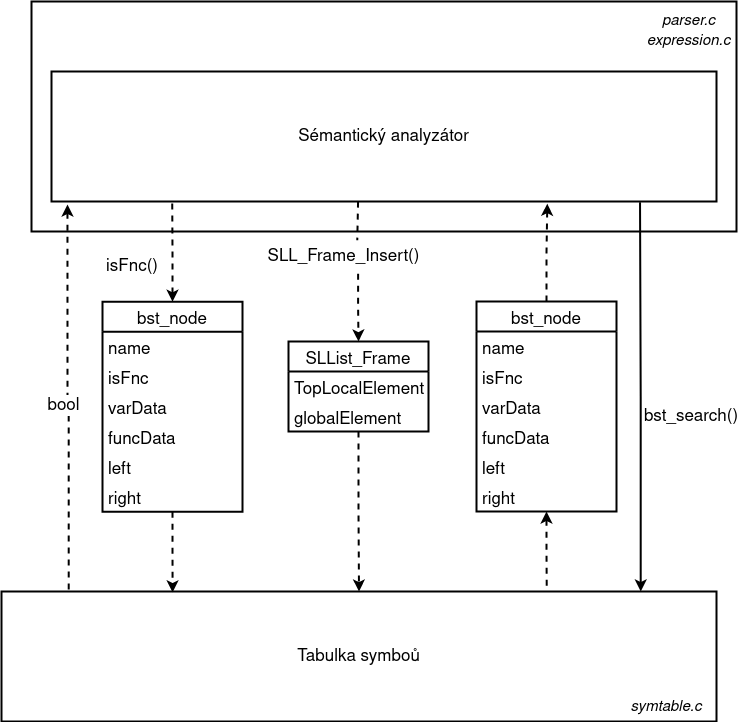
\includegraphics[scale=0.25,keepaspectratio]{img/DiagramSem.png}
    \end{columns}
\end{frame}



\begin{frame}
  \frametitle{Generování kódu}
  \begin{itemize}
        \setlength\itemsep{1em}
            \item Vestavěné funkce v \emph{builtIn.c}
            \item Výpis instrukcí ve funkcích v \emph{generate\_code.c}
            \item Stínění řešeno kopírováním proměnných
            \item Změna této proměnné se vrátí do nižšího rámce
        \end{itemize}
\end{frame}



\begin{frame}
  \frametitle{Práce v týmu}
  \begin{itemize}
    \setlength\itemsep{1em}
        \item Komunikace přes messenger a discord
        \item Github pro hostování repozitáře
        \item Systém \emph{forků a pullrequestů}
        \item Prezenční schůzky na fakultě
    \end{itemize}
    
  \vspace{1em}
    
  \centering
  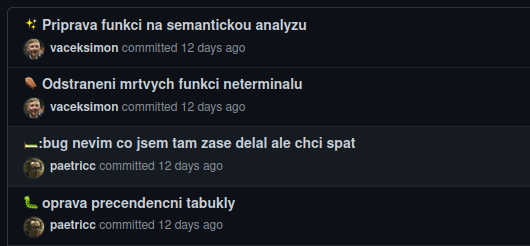
\includegraphics[scale=0.4,keepaspectratio]{img/commit_kekw.png}
\end{frame}


\appendix{}
\begin{frame}
  \frametitle{Děkujeme za pozornost}
    \begin{figure}[htbp]
        \centering
        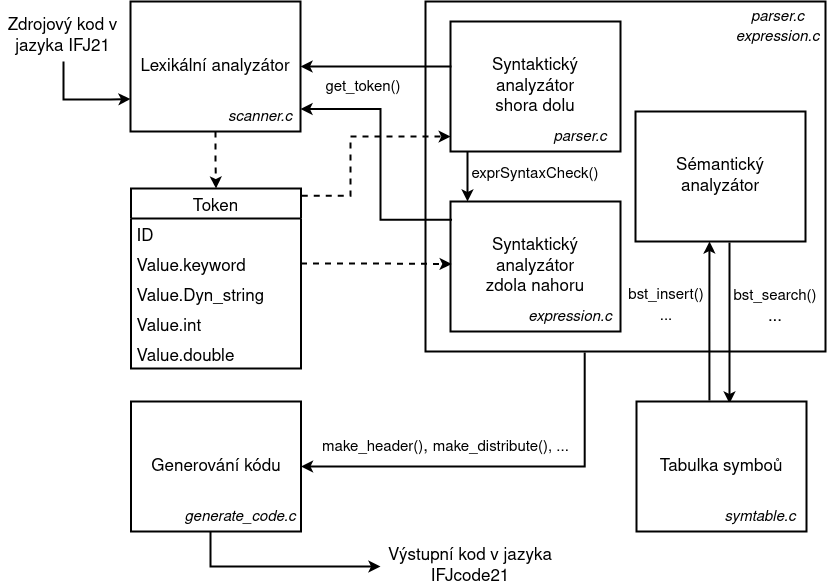
\includegraphics[width=\textwidth,height=\textheight,keepaspectratio]{img/DiagramFinal2.png}
        \label{fig:my_label}
    \end{figure}
 
\end{frame}



\begin{frame} 
  \frametitle{LL tabulka}
  \makebox[\linewidth]{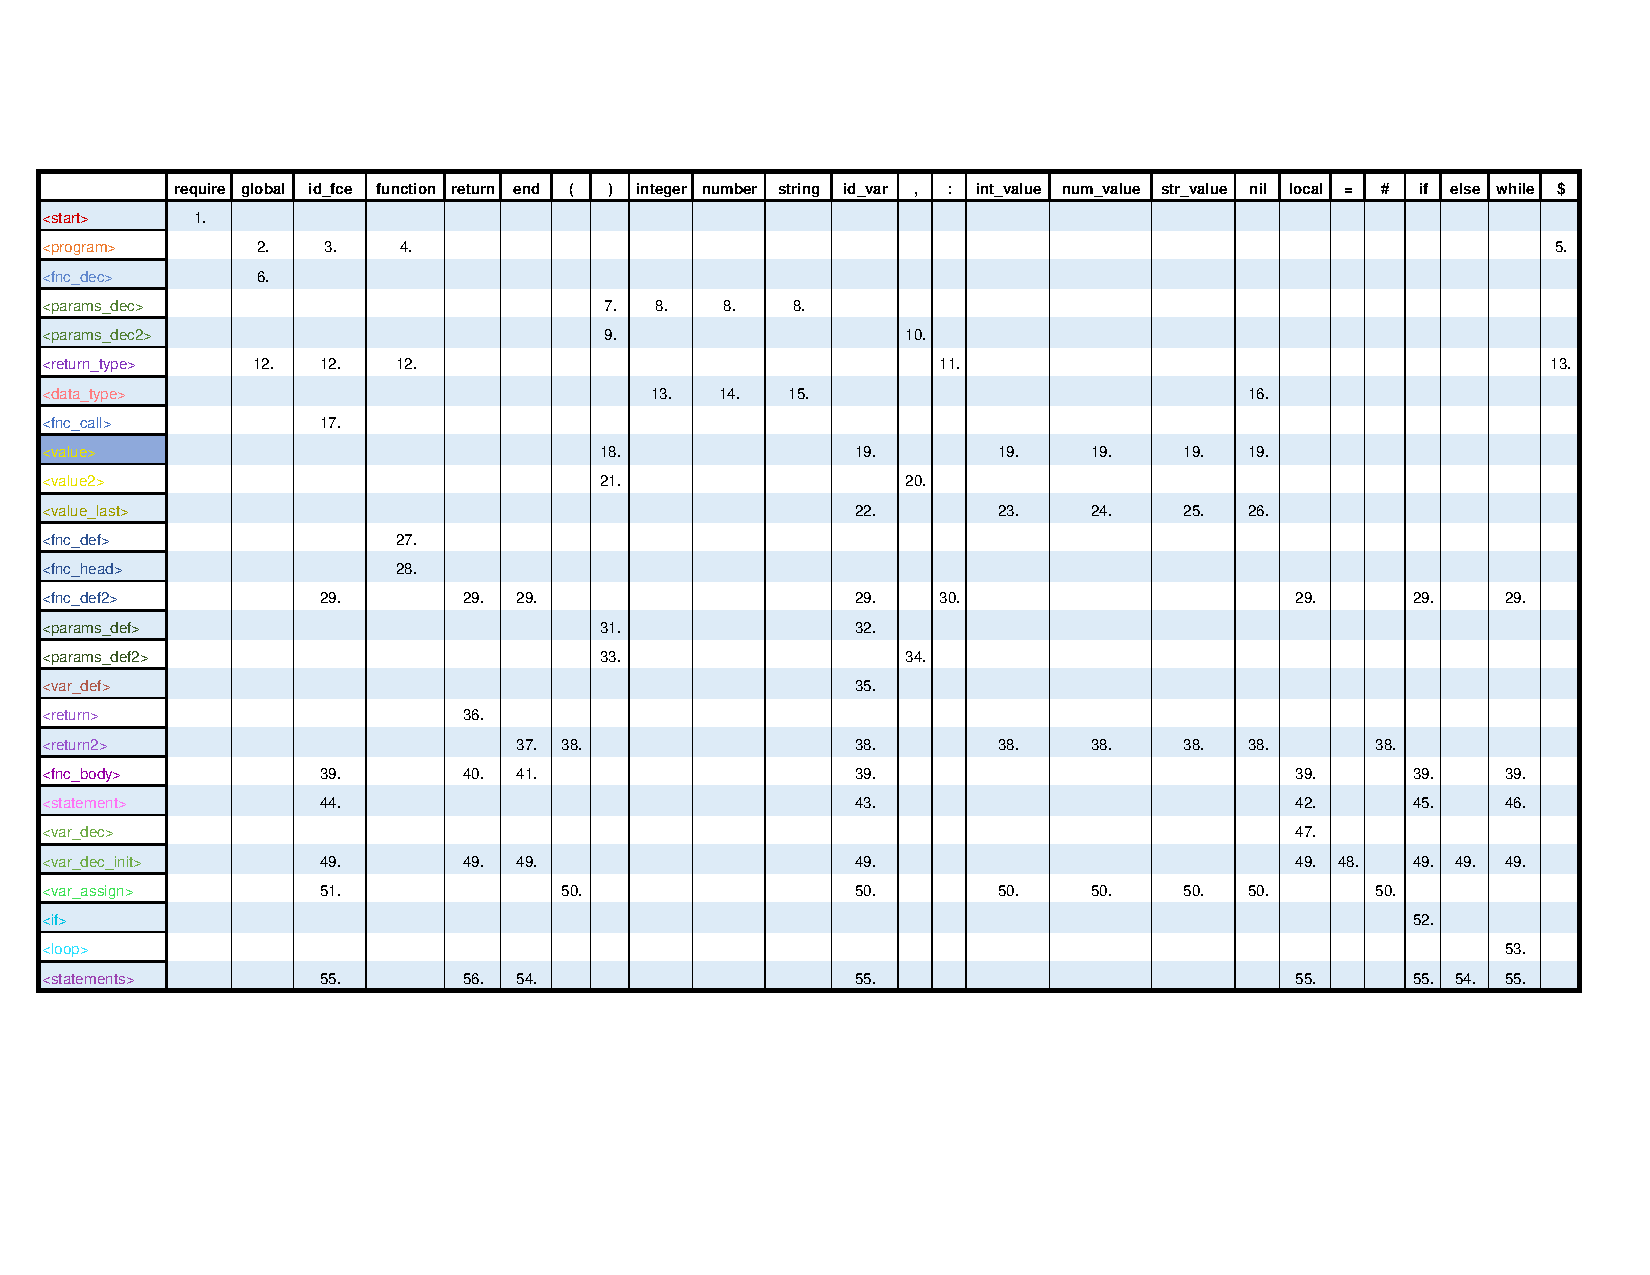
\includegraphics[width=\paperwidth]{img/LLTabulka.pdf}}
\end{frame}


\begin{frame} 
  \frametitle{Precedenční tabulka}
\end{frame}